\subsection{Testläufe}
Im folgenden werden die verschiedenen Testläufe genau beschrieben. Für alle Testläufe gilt, dass das AUV zuerst 30 Meter geradeaus fährt, bevor es auf das Objekt trifft. Dadurch wird eine stabile Fahrt erreicht und die Schwankungen beim anfänglichen Beschleunigen verfälschen die Ergebnisse nicht. Ebenso wird auch gewährleistet, dass das AUV stets direkt auf das Objekt trifft, da das Explorieren und Auffinden des Objektes nicht Teil der Arbeit ist.\\
Zu jedem Testlauf befindet sich auf der CD ein Video, in dem das AUV von oben, sowie die Rohbilder der Kamera, die Ausgabe der Objekterkennung und das berechnete Polynom zu sehen sind.
\subsubsection{Gerader Verlauf}
Für die ersten Tests wurde ein 100 Meter langes Objekt gerade in die Simulationsumgebung eingefügt. Dieses Objekt ist in mehreren Bereichen vom Meeresboden leicht bis komplett bedeckt.\\
Die Testläufe mit geraden Objekten zeigten, dass mit steigender Anzahl an detektierten Punkten die Gerade immer besser vom Schätzverfahren abgebildet wurde. Es sind nach einer längeren geraden Strecke, in der sich das Fahrzeug einpendeln kann, auch weitere Strecken ohne Sichtkontakt kein Problem.\\

\begin{figure}[H]
\begin{tabular}{cc}
\multicolumn{2}{c}{\subfloat[Fahrtverlauf des AUVs (rot) an einem geraden Objekt (blau). Nach erstem Sichtkontakt zum Objekt ist ein Einpendeln auf die gerade Linie zu beobachten.]{\includegraphics[height=0.4\textheight,width=\textwidth]{/testlaeufe/gradeGut/auvroute.jpg}}}\\
\subfloat[Absoluter Fehler der AUV-Position zur echten Position des Objektes. Auch hier ist zu beobachten, dass ein großer Fehler zu Beginn des Objektes auftritt, der beim Fahrtverlauf weiter verringert wird.]{\includegraphics[height=0.3\textheight,width=0.5\textwidth]{/testlaeufe/gradeGut/groundTruthPosition.jpg}}&
\subfloat[Absoluter Fehler der detektierten Objektposition zur echten Objektposition. In Betrachtung von \textit{b)} ist zu beobachten, dass der Fehler der detektierten Objektposition größer ist als der Fehler im daraus resultierenden Fahrtverlauf. Dies ist darauf zurückzuführen, dass es Fehlerausschläge zu beiden Seiten des Objektes gibt, die durch die Regression ausgeglichen werden.]{\includegraphics[height=0.3\textheight,width=0.5\textwidth]{/testlaeufe/gradeGut/groundTruth.jpg}}
\end{tabular}
\caption{Testlauf an einem geraden Objekt. Nach anfänglich größerem Fehler folgt das \gls{auv} dem Objekt mit nur sehr geringem Fehler. Das Einpendeln ist auf die Berechnung des Polynoms zurückzuführen, da bei wenigen Punkten zu Beginn der Verlauf noch nicht eindeutig als Gerade bestimmbar ist. Siehe hierfür Kapitel \ref{sec_pendel}.}
\label{testStraight}
\end{figure}

\subsubsection{Kurve}
Nach den Tests mit geraden Objekten wurden kurvige Objekte mithilfe von Polynomial- und Exponentialfunktionen in die Simulation eingefügt. Hierbei wurde darauf geachtet kein Polynom zweiten Grades zu verwenden, um dem Regressionsverfahren keine perfekte Lösung zu bieten.\\
Ziel dieser Tests ist es zu zeigen, dass das Folgen einer Links- sowie Rechtskurve und auch ein Wechseln zwischen beiden Kurvenarten möglich ist. Für letzteres wurde eine Sinuskurve genutzt, um ein entsprechendes Objekt zu erzeugen.

Außerdem wurde noch eine Kurve nach einer langen Geraden erzeugt. Hiermit wird getestet, ob auch wechselnden geometrischen Strukturen gefolgt werden kann.\\

Bei den Tests mit kurvigen Objekten ist zu beobachten, dass zu Beginn jeder Kurve zunächst ein größerer Fehler zur Objektlage entsteht. Bei lang gezogenen Kurven wird dieser Fehler schnell wieder ausgeglichen. Auch bei mehreren Kurven ist dieses Verhalten zu beobachten (siehe \ref{testSCurve}).


\begin{figure}[H]
\begin{tabular}{cc}
\multicolumn{2}{c}{\subfloat[Fahrtverlauf (rot) bei einer Kurve (blau).]{\includegraphics[height=0.4\textheight,width=\textwidth]{/testlaeufe/linkskurve/auvroute.jpg}}}\\
\subfloat[Fehler der \gls{auv} Position zur echten Position des Objektes. Am Ende ist zu beobachten, wie sich der systematische Fehler aus \textit{c)} in einem beständigen Fehler der Fahrt resultiert.]{\includegraphics[height=0.3\textheight,width=0.5\textwidth]{/testlaeufe/linkskurve/groundTruthPosition.jpg}}&
\subfloat[Fehler der detektierten Objektposition zur echten Objektposition. Es scheint, dass die zweite Hälfte der Punkte einen systematischen Fehler hat. Siehe hierfür Kapitel \ref{sec_sysError}.]{\includegraphics[height=0.3\textheight,width=0.5\textwidth]{/testlaeufe/linkskurve/groundTruth.jpg}}
\end{tabular}
\caption{Testlauf mit einer Kurve. In \textit{a)} und \textit{b)} ist zu erkennen, dass einige Meter benötigt werden, um auf die Kurve zu reagieren. Der zweite größere Fehlerausschlag ist durch eine teilweise komplette Verdeckung des Objektes zu erklären. In \textit{a)} ist sehr gut zu beobachten, dass der Fehler zuerst ansteigt, sobald das Objekt nicht sichtbar ist, bei erneuter Detektion des Objektes aber sehr schnell korrigiert wird.}
\label{fig_leftCurve}
\end{figure}

\begin{figure}[H]
\begin{tabular}{cc}
\multicolumn{2}{c}{\subfloat[Fahrtverlauf (rot) bei einer Kurve (blau).]{\includegraphics[height=0.4\textheight,width=\textwidth]{/testlaeufe/rechtskurveLinks/auvroute.jpg}}}\\
\subfloat[Fehler der \gls{auv} Position zur echten Position des Objektes.]{\includegraphics[height=0.3\textheight,width=0.5\textwidth]{/testlaeufe/rechtskurveLinks/groundTruthPosition.jpg}}&
\subfloat[Fehler der detektierten Objektposition zur echten Objektposition.]{\includegraphics[height=0.3\textheight,width=0.5\textwidth]{/testlaeufe/rechtskurveLinks/groundTruth.jpg}}
\end{tabular}
\caption{Testlauf mit einer Kurve. In diesem Lauf wurde die Kurve, anders als in Abb. \ref{fig_leftCurve}, in die andere Richtung erzeugt. Wie zu erwarten sind die Ergebnisse in diesem Lauf analog zur anderen Kurve.}
\label{fig_rightCurve}
\end{figure}

\begin{figure}[H]
\begin{tabular}{cc}
\multicolumn{2}{c}{\subfloat[Fahrtverlauf (rot) bei einer Kurve nach einer längeren Gerade (blau).]{\includegraphics[height=0.4\textheight,width=\textwidth]{/testlaeufe/gradeKurveSicht/auvroute.jpg}}}\\
\subfloat[Fehler der \gls{auv} Position zur echten Position des Objektes.]{\includegraphics[height=0.3\textheight,width=0.5\textwidth]{/testlaeufe/gradeKurveSicht/groundTruthPosition.jpg}}&
\subfloat[Fehler der detektierten Objektposition zur echten Objektposition.]{\includegraphics[height=0.3\textheight,width=0.5\textwidth]{/testlaeufe/gradeKurveSicht/groundTruth.jpg}}
\end{tabular}
\caption{Testlauf mit einer Kurve nach einer längeren Gerade. In diesem Lauf wird der Wechsel zwischen Gerade und Kurve getestet. Hierbei ist zu sehen, dass die gerade Strecke zunächst gut verfolgt wird. Der Wechsel zur Kurve resultiert in einem größeren Fehler und einem Einpendeln. Dieses Einpendeln fällt stärker aus, da die Parameter so gewählt werden mussten, dass schnell auf Kurven reagiert werden kann (vgl. \ref{sec_param})}
\label{fig_rightCurve}
\end{figure}

\begin{figure}[H]
\begin{tabular}{cc}
\multicolumn{2}{c}{\subfloat[Fahrtverlauf (rot) bei einer Sinuskurve (blau).]{\includegraphics[height=0.4\textheight,width=\textwidth]{/testlaeufe/sinusSicht/auvroute.jpg}}}\\
\subfloat[Fehler der \gls{auv} Position zur echten Position des Objektes. Eine interessante Beobachtung in dieser Grafik ist der sehr ähnliche Fehlerausschlag ]{\includegraphics[height=0.3\textheight,width=0.5\textwidth]{/testlaeufe/sinusSicht/groundTruthPosition.jpg}}&
\subfloat[Fehler der detektierten Objektposition zur echten Objektposition.]{\includegraphics[height=0.3\textheight,width=0.5\textwidth]{/testlaeufe/sinusSicht/groundTruth.jpg}}
\end{tabular}
\caption{Beim Testlauf mit der Sinuskurve ist zu beobachten, dass es innerhalb der Kurven aufgrund der Richtungsänderung des Verlaufs einen größeren Fehler der Verfolgung gibt. Nach der Kurve wird dem Objekt jedoch schnell wieder gut gefolgt.}
\end{figure}

\begin{figure}[H]
\begin{tabular}{cc}
\multicolumn{2}{c}{\subfloat[Fahrtverlauf (rot) bei einem kurvigen Objektverlauf(blau). Da die Kurve zu Beginn einen starken Knick macht, tritt dort ein größerer Fehler auf, bis richtig reagiert wird.]{\includegraphics[height=0.4\textheight,width=\textwidth]{/testlaeufe/S-Kurve_Gut/auvroute.jpg}}}\\
\subfloat[Fehler der \gls{auv} Position zur echten Position des Objektes. Trotz des Fehlers im geraden Bereich und dem sehr großen Fehler innerhalb der Rechtskurve wird das Objekt nach dem Ausschlag wieder gut verfolgt.]{\includegraphics[height=0.3\textheight,width=0.5\textwidth]{/testlaeufe/S-Kurve_Gut/groundTruthPosition.jpg}}&
\subfloat[Fehler der detektierten Objektposition zur echten Objektposition. Der hier zu beobachtende Fehler ist im gesamten Bereich hoch.]{\includegraphics[height=0.3\textheight,width=0.5\textwidth]{/testlaeufe/S-Kurve_Gut/groundTruth.jpg}}
\end{tabular}
\caption{Den Kurven in diesem Lauf ist für das \gls{auv} aufgrund der starken Krümmung schwer zu folgen. Im mittleren Bereich tritt auf längerer Strecke ein größerer Fehler auf. Aufgrund dieses Fehlers wird die Rechtskurve fast \textit{verpasst} jedoch aufgrund des Schätzverfahrens trotzdem noch verfolgt. In diesem Lauf ist der Zusammenhang zwischen Positions- und Detektionsfehler deutlich zu erkennen.}
\label{testSCurve}
\end{figure}

\subsubsection{Ellipsen}
Für die finalen Tests wurden Ellipsen verwendet. Eine Ellipse erfüllt einige Eigenschaften, die für die Arbeit zu nicht trivial zu lösenden Problemen führen. Zum einen gibt es verschieden stark gebogene Kurven und fast gerade Abschnitte. Zum anderen gibt es kontinuierliche Abschnitte, die parallel zur $Y-Achse$ verlaufen.\\
In diesen Tests ist zu sehen, dass sowohl Ellipsen, als auch der Wechsel zwischen Geraden und Ellipsenabschnitten gefolgt werden kann.

\begin{figure}[H]
\begin{tabular}{cc}
\multicolumn{2}{c}{\subfloat[Fahrtverlauf (rot) bei einer Ellipse (blau). Es wurde anderthalb mal um die Ellipse gefahren.]{\includegraphics[height=0.4\textheight,width=\textwidth]{/testlaeufe/kreissicht/auvroute.jpg}}}\\
\subfloat[Fehler der \gls{auv} Position zur echten Position des Objektes. Es ist ein gleichmäßiges Auftreten von Fehlerspitzen zu beobachten. Der größte Ausschlag ist einer Unsichtbarkeit des Objektes innerhalb des rechten oberen Ellipsenabschnitts zuzuschreiben.]{\includegraphics[height=0.3\textheight,width=0.5\textwidth]{/testlaeufe/kreissicht/groundTruthPosition.jpg}}&
\subfloat[Fehler der detektierten Objektposition zur echten Objektposition. Es sind zwei Bereiche mit größerem Fehler zu beobachten. Diese liegen beide im unteren linken Bereich der Ellipse, in dem das Objekt teilweise vom Meeresboden bedeckt ist.]{\includegraphics[height=0.3\textheight,width=0.5\textwidth]{/testlaeufe/kreissicht/groundTruth.jpg}}
\end{tabular}
\caption{Im Testlauf der Ellipse ist zu beobachten, wie die ständig ändernde Krümmung der Bahn zu Fehlerspitzen führt. Bei jeder Spitze ist der Fehler der Regression so hoch, dass eine \gls{transform} der detektierten Punkte stattfindet (siehe Kapitel \ref{sec_curveFit}), die zu einer direkten Abnahme des Fehlers führt.}
\end{figure}

\begin{figure}[H]
\begin{tabular}{cc}
\multicolumn{2}{c}{\subfloat[Fahrtverlauf (rot) bei einer Ellipse mit geraden Abschnitten (blau).]{\includegraphics[height=0.4\textheight,width=\textwidth]{/testlaeufe/gradeKreissicht/auvroute.jpg}}}\\
\subfloat[Fehler der \gls{auv} Position zur echten Position des Objektes.]{\includegraphics[height=0.3\textheight,width=0.5\textwidth]{/testlaeufe/gradeKreissicht/groundTruthPosition.jpg}}&
\subfloat[Fehler der detektierten Objektposition zur echten Objektposition.]{\includegraphics[height=0.3\textheight,width=0.5\textwidth]{/testlaeufe/gradeKreissicht/groundTruth.jpg}}
\end{tabular}
\caption{Testlauf von einer Ellipse gemischt mit geraden Abschnitten. Beim Übergang in die Ellipse ist ein erwarteter hoher Fehler zu beobachten, der durch den Wechsel der Form zu erklären ist. Innerhalb der Ellipse sind einige verdeckte Bereiche, was die Fehler in \textit{b)} und \textit{c)} erklärt.}
\label{testStraightCirc}
\end{figure}

\subsubsection{Schlechte Sichtbedingungen}
Einige Tests wurden mit sehr schlechten Sichtbedingungen (siehe Abb. \ref{img_badSeight}) wiederholt. In den Tests ist zu sehen, dass selbst unter diesen Bedingungen dem Objekt gefolgt werden kann. Jedoch ist bei diesen Tests zu beachten, dass der Templateschwellenwert sehr gering gewählt wurde und dadurch eine sehr sensitive Objekterkennung genutzt wurde. Da jedoch in der Simulation nur Meeresboden und Zielobjekt existieren führte dies nicht zu Problemen. Schon kleinste Objekte, wie kleinere Felsen oder Pflanzen, würden bei einem solch geringen Schwellenwert zu schwerwiegenden Fehldetektionen führen. Tests mit anderen Objekten in der Simulationsumgebung wurden jedoch nicht durchgeführt, da es keine einfache Methode gibt Steine oder Pflanzen hinzuzufügen. Die Tatsache, dass aber selbst der Meeresboden schon zu Störpunkten innerhalb des Binärbilds führt unterstützt diese Aussage.

\begin{figure}[H]
\begin{tabular}{cc}
\multicolumn{2}{c}{\subfloat[Fahrtverlauf des \gls{auv}s (rot) bei einer Kurve (blau) unter schlechten Sichtbedingungen. ]{\includegraphics[height=0.4\textheight,width=\textwidth]{/testlaeufe/linkskurveschlechtesicht/auvroute.jpg}}}\\
\subfloat[Fehler der \gls{auv} Position zur echten Position des Objektes.]{\includegraphics[height=0.3\textheight,width=0.5\textwidth]{/testlaeufe/linkskurveschlechtesicht/groundTruthPosition.jpg}}&
\subfloat[Fehler der detektierten Objektposition zur echten Objektposition. Der Anstieg zum Ende ist auf leichte Verdeckung des Objektes zurückzuführen.]{\includegraphics[height=0.3\textheight,width=0.5\textwidth]{/testlaeufe/linkskurveschlechtesicht/groundTruth.jpg}}
\end{tabular}
\caption{Das Folgen der Kurve funktioniert auch bei schlechten Sichtbedingungen. Es ist jedoch zu beobachten, dass eine nur leichte Verdeckung des Objektes einen starken Einfluss auf den Fehler hat.}
\label{curveBadSight}
\end{figure}

\begin{figure}[H]
\begin{tabular}{cc}
\multicolumn{2}{c}{\subfloat[Fahrtverlauf (rot) bei einer Ellipse (blau) unter schlechten Sichtbedingungen.]{\includegraphics[height=0.4\textheight,width=\textwidth]{/testlaeufe/kreisschlechtesicht/auvroute.jpg}}}\\
\subfloat[Fehler der \gls{auv} Position zur echten Position des Objektes.]{\includegraphics[height=0.3\textheight,width=0.5\textwidth]{/testlaeufe/kreisschlechtesicht/groundTruthPosition.jpg}}&
\subfloat[Fehler der detektierten Objektposition zur echten Objektposition.]{\includegraphics[height=0.3\textheight,width=0.5\textwidth]{/testlaeufe/kreisschlechtesicht/groundTruth.jpg}}
\end{tabular}
\caption{Ähnlich zu Abb. \ref{curveBadSight} wird dem Objekt gut gefolgt und leichte Verdeckungen haben einen starken Einfluss auf den Fehler.}
\end{figure}